\documentclass[11pt,a4paper]{article}
\usepackage[utf8]{inputenc}
\usepackage[T1]{fontenc}
\usepackage{amsmath,amssymb,amsfonts}
\usepackage{amsthm}
\usepackage[margin=2.5cm]{geometry}
\usepackage{enumitem}
\usepackage{tikz}
\usepackage{xcolor}
\usepackage{hyperref}
\hypersetup{colorlinks=true,linkcolor=blue!55!black,urlcolor=blue!55!black}
\setlist[itemize]{leftmargin=1.4em,itemsep=2pt,topsep=3pt}

% ── theorem environments (numbered, standard) ──
\newtheorem{theorem}{Theorem}[section]
\newtheorem{lemma}[theorem]{Lemma}
\newtheorem{proposition}[theorem]{Proposition}
\newtheorem{corollary}[theorem]{Corollary}
\theoremstyle{definition}
\newtheorem{definition}[theorem]{Definition}
\newtheorem{example}[theorem]{Example}
\newtheorem{remark}[theorem]{Remark}
\newtheorem{exercise}{Exercise}

% ── master macro block (safe, multi-character) ──
\newcommand{\Z}{\mathbb{Z}}
\newcommand{\Q}{\mathbb{Q}}
\newcommand{\R}{\mathbb{R}}
\newcommand{\C}{\mathbb{C}}
\newcommand{\N}{\mathbb{N}}
\newcommand{\F}{\mathbb{F}}
\newcommand{\Spec}{\operatorname{Spec}}
\newcommand{\diam}{\operatorname{diam}}

\title{
	{\color{blue!40!black}\textbf{\Huge Point}}\\[0.3em]
	\Large \textit{From Number Theory to Algebraic Geometry and Logic}\\[0.7em]
	\large \textbf{Session P2 --- Topology and Metric Spaces}\\[0.3em]
	\normalsize \emph{Complete lecture notes with proofs, examples, and exercises}
}
\author{}
\date{}

\begin{document}
	\maketitle
	\thispagestyle{empty}
	
	\begin{abstract}
		\noindent
		This session builds the language of \emph{closeness}. Two machines are constructed and proved
		correct, because the entire course runs on them: \textbf{compactness} (which turns open covers into
		finite data --- the engine behind adelic finiteness in S22 and profinite compactness in S34) and
		\textbf{completion} (which adds exactly the points that Cauchy sequences deserved --- the machine
		that turns $\Q$ into $\R$ here and into $\Q_p$ in S17--S18). Along the way: bases, subspace and
		product topologies (with the infinite-product remark that previews the restricted product of
		adeles), connectedness of intervals, the Heine--Borel picture, Hausdorffness, and the equivalence
		of $\varepsilon$--$\delta$ and open-set continuity.
	\end{abstract}
	
	\subsection*{Session plan (150 minutes)}
	\begin{center}\small
		\begin{tabular}{|l|l|}
			\hline
			\textbf{Time} & \textbf{Block} \\
			\hline
			0:00--0:10 & Orientation: closeness without distance; where topology returns (S1 Zariski, S17--S22, S34, S38) \\
			0:10--0:35 & \S1 Topological spaces: axioms, bases, subspace \& product, continuity, homeomorphism \\
			0:35--1:00 & \S1 cont.: connectedness of intervals; compactness of the unit interval; Hausdorff \\
			1:00--1:10 & \emph{Break} \\
			1:10--1:35 & \S2 Metric spaces: balls as a basis; $\varepsilon$--$\delta$ $\iff$ open-set continuity; Cauchy; completeness \\
			1:35--2:05 & \S3 Completion: construction, completeness, density, uniqueness; $\Q\to\R$; preview $\Q\to\Q_p$, Ostrowski \\
			2:05--2:20 & \S4 Compactness in metric spaces; uniform continuity; extreme values \\
			2:20--2:30 & Wrap-up: completion $=$ adding missing points; bridge to S17--S22 \\
			\hline
		\end{tabular}
	\end{center}
	
	\subsection*{Conventions}
	All spaces are nonempty unless stated. ``Open'' always means open in the topology under
	discussion; subspace and product topologies are defined explicitly when used. In metric contexts
	$d$ denotes the metric and $B(x,r)=\{y:d(x,y)<r\}$ the open ball. Sequences are written
	$(x_n)_{n\ge1}$ or $(x_n)$.
	
	\tableofcontents
	\newpage
	
	% ══════════════════════════════════════════════
	\section{Topological Spaces}
	% ══════════════════════════════════════════════
	
	\begin{definition}[Topology]
		A \textbf{topology} on a set $X$ is a collection $\tau\subseteq\mathcal P(X)$ of \textbf{open sets} with:
		\begin{enumerate}[label=(T\arabic*)]
			\item $\varnothing\in\tau$ and $X\in\tau$;
			\item arbitrary unions of members of $\tau$ lie in $\tau$;
			\item finite intersections of members of $\tau$ lie in $\tau$.
		\end{enumerate}
		A set is \textbf{closed} if its complement is open. The pair $(X,\tau)$ is a \textbf{topological space}.
	\end{definition}
	
	\begin{example}[First examples]\label{ex:topologies}
		\begin{itemize}
			\item \textbf{Discrete:} $\tau=\mathcal P(X)$. Every subset open (and closed).
			\item \textbf{Indiscrete:} $\tau=\{\varnothing,X\}$.
			\item \textbf{Standard on $\R$:} $\tau$ generated by open intervals $(a,b)$ (made precise by
			Proposition~\ref{prop:basis}); equivalently the metric topology of $|x-y|$ (\S2).
			\item \textbf{Cofinite:} $\tau=\{\varnothing\}\cup\{U:X\setminus U\text{ finite}\}$ on any infinite $X$
			(check (T2),(T3): unions of cofinite are cofinite; intersections of finitely many cofinite are cofinite).
			\item \textbf{Zariski:} on $\Spec R$ (Session~S1) and on $k^n$ (zero sets of polynomials closed);
			recall it is \emph{not} Hausdorff --- Remark~\ref{rem:zariski-not-hausdorff}.
		\end{itemize}
	\end{example}
	
	\begin{definition}[Basis]
		A \textbf{basis} for a topology on $X$ is a collection $\mathcal B\subseteq\mathcal P(X)$ with:
		\begin{enumerate}[label=(B\arabic*)]
			\item $\bigcup_{B\in\mathcal B}B=X$;
			\item if $x\in B_1\cap B_2$ with $B_i\in\mathcal B$, then $\exists B_3\in\mathcal B$ with $x\in B_3\subseteq B_1\cap B_2$.
		\end{enumerate}
	\end{definition}
	
	\begin{proposition}[A basis generates a topology]\label{prop:basis}
		If $\mathcal B$ satisfies (B1),(B2), then
		\[
		\tau=\Big\{U\subseteq X:\ \forall x\in U\ \exists B\in\mathcal B,\ x\in B\subseteq U\Big\}
		\]
		is a topology, and $\tau$ is exactly the set of unions of members of $\mathcal B$.
	\end{proposition}
	\begin{proof}
		$\varnothing\in\tau$ vacuously; $X\in\tau$ by (B1). Unions: if $x\in\bigcup_i U_i$ then $x\in U_j$ for
		some $j$, so a witness $B$ for $U_j$ witnesses $\bigcup_i U_i$. Intersections: if
		$x\in U_1\cap U_2$ with witnesses $B_1,B_2$, then (B2) gives $B_3$ with $x\in B_3\subseteq B_1\cap B_2
		\subseteq U_1\cap U_2$. Every union of basis elements is in $\tau$ (each point witnessed by its own
		$B$); conversely each $U\in\tau$ equals $\bigcup\{B\in\mathcal B:B\subseteq U\}$ by definition.
	\end{proof}
	
	\begin{definition}[Subspace topology]
		For $Y\subseteq X$, the \textbf{subspace topology} on $Y$ has as opens exactly $\{U\cap Y:U\in\tau_X\}$.
	\end{definition}
	
	\begin{example}
		In $Y=(0,1]\subseteq\R$ the set $(\tfrac12,1]$ is \emph{open} (it is $(\tfrac12,2)\cap Y$) although it
		is not open in $\R$. In $Y=\Z\subseteq\R$ every subset is open (discrete subspace), since
		$\{n\}=(n-\tfrac12,n+\tfrac12)\cap\Z$.
	\end{example}
	
	\begin{definition}[Product topology]
		On $X\times Y$, the \textbf{product topology} has basis $\{U\times V:U\in\tau_X,\ V\in\tau_Y\}$
		(the basis axioms hold trivially). For finitely many factors, basis $\prod_i U_i$.
	\end{definition}
	
	\begin{remark}[Infinite products, and a preview of adeles]\label{rem:infinite-product}
		For an infinite family $\prod_i X_i$, the \textbf{product topology} takes as basis the sets
		$\prod_i U_i$ with $U_i$ open and $U_i=X_i$ for \emph{all but finitely many} $i$; the \textbf{box
			topology} drops this restriction and is too fine (products of compact spaces fail to be compact,
		etc.). The ``all but finitely many'' discipline returns in Session~S22: the adele ring
		$\mathbb A_\Q$ is a \emph{restricted} product, $\{(x_v)_v:x_p\in\Z_p\text{ for all but finitely many }p\}$
		--- the same philosophy of controlled infinity, now arithmetic.
	\end{remark}
	
	\begin{definition}[Continuity; homeomorphism]
		$f:X\to Y$ is \textbf{continuous} if $f^{-1}(V)$ is open for every open $V\subseteq Y$. A
		\textbf{homeomorphism} is a bijective continuous map with continuous inverse; then $X\cong Y$
		topologically.
	\end{definition}
	
	\begin{proposition}
		Compositions of continuous maps are continuous; identities are continuous; a bijection $f$ is a
		homeomorphism $\iff$ $f^{-1}(V)$ open $\iff$ $f(U)$ open for all opens.
	\end{proposition}
	
	\begin{example}
		$\tan$ gives $(0,1)\cong\R$ (rescaled). The map $[0,1)\to S^1$, $t\mapsto e^{2\pi i t}$, is continuous
		and bijective but \emph{not} a homeomorphism (its inverse is discontinuous at $1$; compactness will
		explain this cleanly, Corollary~\ref{cor:compact-invariants}).
	\end{example}
	
	\begin{definition}[Connected]
		$X$ is \textbf{disconnected} if $X=U\sqcup V$ with $U,V$ nonempty open; otherwise \textbf{connected}.
	\end{definition}
	
	\begin{proposition}\label{prop:connected-image}
		The continuous image of a connected space is connected.
	\end{proposition}
	\begin{proof}
		If $f(X)=U\sqcup V$ is a disconnection then $X=f^{-1}(U)\sqcup f^{-1}(V)$ is a disconnection of $X$
		(preimages of opens are open, disjoint, and cover since $U,V$ cover $f(X)$).
	\end{proof}
	
	\begin{theorem}[Intervals are connected]\label{thm:intervals-connected}
		Every interval $I\subseteq\R$ (in the standard topology) is connected; in particular $\R$ and the
		unit interval are connected.
	\end{theorem}
	\begin{proof}
		Suppose $I=U\sqcup V$ with $U,V$ nonempty open in $I$. Pick $a\in U$, $b\in V$; wlog $a<b$; replace
		$I$ by $[a,b]\subseteq I$ and $U,V$ by their intersections with $[a,b]$ (still a disconnection,
		$a\in U$, $b\in V$). Let $s=\sup(U\cap[a,b])$; then $s\in[a,b]=U\sqcup V$.
		
		If $s\in U$: $U$ open in $[a,b]$ gives $\varepsilon>0$ with $[s,s+\varepsilon)\subseteq U$ when $s<b$;
		then $s+\varepsilon/2\in U$ exceeds the supremum --- impossible; and $s=b$ forces $b\in U\cap V$.
		
		If $s\in V$: $V$ open gives $\varepsilon>0$ with $(s-\varepsilon,s]\subseteq V$; but $s$ being the
		\emph{least} upper bound of $U\cap[a,b]$ yields $u\in U\cap(a,s]\subseteq U\cap V$ --- impossible.
		Both cases fail, so no disconnection exists.
	\end{proof}
	
	\begin{example}
		$\Q$ is \textbf{totally disconnected}: for $x<y$ in $\Q$ pick an irrational $t\in(x,y)$; then
		$(-\infty,t)\cap\Q$ and $(t,\infty)\cap\Q$ disconnect any subset containing $x,y$. Also
		$[0,1]\sqcup[2,3]$ is disconnected. Contrast: $\R_{>0}$, circles, and all intervals are connected.
	\end{example}
	
	\begin{definition}[Compact]
		$X$ is \textbf{compact} if every open cover $\{U_i\}_{i\in I}$ of $X$ has a finite subcover.
	\end{definition}
	
	\begin{example}\label{ex:compact}
		\begin{itemize}
			\item Finite spaces are compact; $\{1/n:n\ge1\}\cup\{0\}\subseteq\R$ is compact (any cover: one open
			catches $0$ and hence all but finitely many points).
			\item $(0,1)$ is \emph{not} compact: $(1/n,1)_{n\ge2}$ covers with no finite subcover.
			\item $\R$ is not compact: $(-n,n)_{n\ge1}$ covers with no finite subcover.
			\item The unit interval \emph{is} compact: Theorem~\ref{thm:01-compact}.
		\end{itemize}
	\end{example}
	
	\begin{proposition}[Continuous images of compact sets]\label{prop:compact-image}
		The continuous image of a compact space is compact.
	\end{proposition}
	\begin{proof}
		If $\{V_i\}$ covers $f(X)$ then $\{f^{-1}(V_i)\}$ covers $X$; a finite subcover of the latter maps to
		a finite subcover of the former.
	\end{proof}
	
	\begin{theorem}[Compactness of the unit interval]\label{thm:01-compact}
		The interval $[0,1]$, with the standard topology, is compact.
	\end{theorem}
	\begin{proof}[Proof by bisection]
		Assume an open cover $\mathcal U$ with no finite subcover. Bisect: of the two halves of $[0,1]$, at
		least one cannot be finitely covered (else the union could); call it $I_1$. Bisect $I_1$, choose a
		non-finitely-coverable half $I_2$; continue, obtaining nested closed intervals $I_n$ with
		$|I_n|=2^{-n}$, none finitely covered. By the nested-interval property, $\bigcap_n I_n=\{s\}$ for a
		single $s\in[0,1]$. Some $U\in\mathcal U$ contains $s$, and $U$ open gives $\varepsilon>0$ with
		$(s-\varepsilon,s+\varepsilon)\cap[0,1]\subseteq U$. Choose $n$ with $2^{-n}<\varepsilon$; since
		$s\in I_n$ and $|I_n|<\varepsilon$, $I_n\subseteq(s-\varepsilon,s+\varepsilon)$, so $\{U\}$ finitely
		covers $I_n$ --- contradiction.
	\end{proof}
	
	\begin{figure}[h]
		\centering
		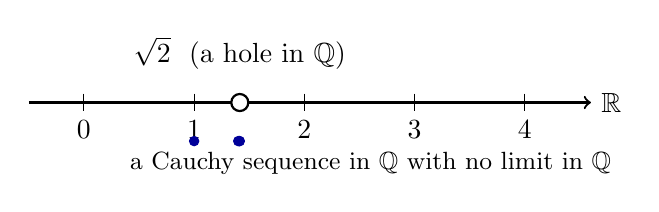
\begin{tikzpicture}[scale=1.4]
			\draw[thick,->] (-0.5,0) -- (4.6,0) node[right] {$\R$};
			\foreach \x/\l in {0/0,1/1,2/2,3/3,4/4} {\draw (\x,0.08) -- (\x,-0.08) node[below] {$\l$};}
			\draw[fill=white,thick] (1.4142,0) circle (2.2pt);
			\node at (1.4142,0.45) {$\sqrt2$ \ (a hole in $\Q$)};
			\foreach \n/\x in {1/1,2/1.4,3/1.41,4/1.414} {\filldraw[blue!60!black] (\x,-0.35) circle (1.2pt);}
			\node at (2.6,-0.55) {\small a Cauchy sequence in $\Q$ with no limit in $\Q$};
		\end{tikzpicture}
		\caption{Incompleteness as a \emph{missing point}: the rationals have a hole exactly where a Cauchy
			sequence demands a limit. Completion (\S3) fills all such holes at once.}
	\end{figure}
	
	\begin{proposition}[Closed inside compact; Heine--Borel for $\R$]\label{prop:heine-borel}
		\begin{enumerate}[label=(\alph*)]
			\item A closed subset of a compact space is compact.
			\item (Heine--Borel, $n=1$) $K\subseteq\R$ is compact $\iff$ $K$ is closed and bounded.
		\end{enumerate}
	\end{proposition}
	\begin{proof}
		(a) If $K\subseteq X$ closed and $\{U_i\}$ covers $K$, then $\{U_i\}\cup\{X\setminus K\}$ covers $X$;
		a finite subcover minus $X\setminus K$ finitely covers $K$. (b) ($\Leftarrow$) Bounded gives
		$K\subseteq[a,b]$; $[a,b]$ is homeomorphic to $[0,1]$ (rescaling), hence compact
		(Theorem~\ref{thm:01-compact}); closed-in-compact gives $K$ compact by (a). ($\Rightarrow$) Compact
		$K$ is bounded since $(-n,n)_n$ must admit a finite subcover; and $K$ is closed by
		Proposition~\ref{prop:hausdorff}(b).
	\end{proof}
	
	\begin{definition}[Hausdorff]
		$X$ is \textbf{Hausdorff} ($T_2$) if distinct points have disjoint open neighbourhoods.
	\end{definition}
	
	\begin{proposition}[Hausdorff consequences]\label{prop:hausdorff}
		\begin{enumerate}[label=(\alph*)]
			\item Limits of sequences are unique in Hausdorff spaces.
			\item Compact subsets of Hausdorff spaces are closed.
		\end{enumerate}
	\end{proposition}
	\begin{proof}
		(a) If $x_n\to x$ and $x_n\to y$ with $x\neq y$, disjoint $U\ni x$, $V\ni y$ force $x_n\in U\cap V=\varnothing$
		for large $n$. (b) Let $K$ compact in Hausdorff $X$; for $x\notin K$, each $y\in K$ has disjoint
		$U_y\ni x$, $V_y\ni y$; finitely many $V_{y_i}$ cover $K$; then $U=\bigcap_i U_{y_i}$ is an open
		neighbourhood of $x$ disjoint from $K$; so $X\setminus K$ is open.
	\end{proof}
	
	\begin{corollary}\label{cor:compact-invariants}
		Compactness is a homeomorphism invariant; hence $[0,1]\not\cong(0,1)\not\cong\R$, and
		the bijection $[0,1)\to S^1$ of the example above is not a homeomorphism.
	\end{corollary}
	
	\begin{remark}[Zariski is not Hausdorff]\label{rem:zariski-not-hausdorff}
		In $\Spec\Z$ (Session~S1) any two nonempty opens meet: $D(m)\cap D(n)=D(mn)\neq\varnothing$. So the
		Zariski topology sacrifices Hausdorffness to remember \emph{algebraic} specialization; the metric and
		\'etale topologies (S17--, S52) restore separation where it is needed.
	\end{remark}
	
	% ══════════════════════════════════════════════
	\section{Metric Spaces}
	% ══════════════════════════════════════════════
	
	\begin{definition}[Metric]
		A \textbf{metric} on $X$ is $d:X\times X\to\R_{\ge0}$ with: $d(x,y)=0\iff x=y$; symmetry
		$d(x,y)=d(y,x)$; triangle inequality $d(x,z)\le d(x,y)+d(y,z)$.
	\end{definition}
	
	\begin{example}\label{ex:metrics}
		\begin{itemize}
			\item Euclidean $d_2(x,y)=\big(\sum_i(x_i-y_i)^2\big)^{1/2}$ on $\R^n$; taxicab $d_1=\sum_i|x_i-y_i|$;
			max metric $d_\infty=\max_i|x_i-y_i|$ (all give the standard topology on $\R^n$).
			\item Discrete metric: $d(x,y)=1$ for $x\neq y$; induces the discrete topology.
			\item Sup metric on $C[0,1]$: $d_{\sup}(f,g)=\sup_{t\in[0,1]}|f(t)-g(t)|$; convergence $=$ uniform convergence.
			\item Preview (S17): the $p$-adic metric $d_p(x,y)=p^{-v_p(x-y)}$ on $\Q$; ultrametric inequality
			$d_p(x,z)\le\max\{d_p(x,y),d_p(y,z)\}$ --- a geometry where all triangles are isosceles (S19).
		\end{itemize}
	\end{example}
	
	\begin{proposition}[Balls form a basis]\label{prop:balls-basis}
		The open balls $B(x,r)$ satisfy (B1),(B2); hence every metric space carries a canonical
		\textbf{metric topology}.
	\end{proposition}
	\begin{proof}
		(B1): $x\in B(x,1)$. (B2): if $z\in B(x,r)\cap B(y,s)$ set $\varepsilon=\min\{r-d(x,z),\,s-d(y,z)\}>0$;
		then for $w\in B(z,\varepsilon)$: $d(x,w)\le d(x,z)+d(z,w)<d(x,z)+\varepsilon\le r$, so
		$B(z,\varepsilon)\subseteq B(x,r)$; symmetrically for $B(y,s)$.
	\end{proof}
	
	\begin{proposition}
		Every metric space is Hausdorff; hence limits of sequences are unique.
	\end{proposition}
	\begin{proof}
		For $x\neq y$, $r=d(x,y)/2$ gives disjoint $B(x,r)$, $B(y,r)$ (triangle inequality). Then apply
		Proposition~\ref{prop:hausdorff}(a).
	\end{proof}
	
	\begin{definition}[Convergence; Cauchy; completeness]
		$x_n\to x$ means $\forall\varepsilon>0\ \exists N\ \forall n\ge N:\ d(x_n,x)<\varepsilon$.
		$(x_n)$ is \textbf{Cauchy} if $\forall\varepsilon>0\ \exists N\ \forall m,n\ge N:\ d(x_m,x_n)<\varepsilon$.
		$(X,d)$ is \textbf{complete} if every Cauchy sequence converges in $X$.
	\end{definition}
	
	\begin{proposition}\label{prop:conv-cauchy}
		Every convergent sequence is Cauchy.
	\end{proposition}
	\begin{proof}
		Given $\varepsilon$, choose $N$ with $d(x_n,x)<\varepsilon/2$ for $n\ge N$; then
		$d(x_m,x_n)\le d(x_m,x)+d(x,x_n)<\varepsilon$.
	\end{proof}
	
	\begin{example}[Incompleteness as missing points]
		In $\Q$: the decimals $1,1.4,1.41,1.414,\dots$ of $\sqrt2$ are Cauchy (they converge in $\R$, use
		Proposition~\ref{prop:conv-cauchy}) but have no limit in $\Q$ (no rational squares to $2$). In
		$(0,1)$: $x_n=1/n$ is Cauchy with no limit in the space. In both cases a \emph{point is missing}
		(Figure~1).
	\end{example}
	
	\begin{theorem}[Completeness of the sup metric]\label{thm:C-complete}
		The metric space $(C[0,1], d_{\sup})$ is complete: every Cauchy sequence of continuous functions
		converges uniformly to a continuous function.
	\end{theorem}
	\begin{proof}
		Let $(f_n)$ be Cauchy. For each $t$, $(f_n(t))$ is Cauchy in $\R$ (since
		$|f_m(t)-f_n(t)|\le d_{\sup}(f_m,f_n)$), hence converges; define $f(t)=\lim_n f_n(t)$. Uniformity:
		given $\varepsilon$, choose $N$ with $d_{\sup}(f_m,f_n)<\varepsilon$ for $m,n\ge N$; fixing $n\ge N$
		and letting $m\to\infty$ gives $|f(t)-f_n(t)|\le\varepsilon$ for all $t$, so $d_{\sup}(f,f_n)\le\varepsilon$:
		$f_n\to f$ uniformly. Continuity of $f$: for $t_0$ and $\varepsilon$, pick $n$ with
		$d_{\sup}(f,f_n)<\varepsilon/3$, then $\delta$ with $|f_n(t)-f_n(t_0)|<\varepsilon/3$ for
		$|t-t_0|<\delta$; then $|f(t)-f(t_0)|\le|f(t)-f_n(t)|+|f_n(t)-f_n(t_0)|+|f_n(t_0)-f(t_0)|<\varepsilon$.
	\end{proof}
	
	\begin{proposition}\label{prop:complete-closed}
		In a complete metric space, a subspace is complete $\iff$ it is closed. In particular complete
		subspaces of complete spaces are closed, and closed subspaces of complete spaces are complete.
	\end{proposition}
	\begin{proof}
		If $Y$ complete and $x_n\to x$ with $x_n\in Y$, then $(x_n)$ Cauchy in $Y$, so converges in $Y$ to
		some $y\in Y$; uniqueness of limits gives $x=y\in Y$: $Y$ closed. Conversely if $Y$ closed and
		$(x_n)$ Cauchy in $Y$, it converges in $X$ to some $x$; closedness forces $x\in Y$: convergence in $Y$.
	\end{proof}
	
	\begin{theorem}[Epsilon--delta versus open sets]\label{thm:eps-delta}
		For $f:X\to Y$ between metric spaces, the following are equivalent:
		\begin{enumerate}[label=(\alph*)]
			\item $f$ is continuous in the open-set sense;
			\item $f$ is continuous at every point: $\forall x\ \forall\varepsilon>0\ \exists\delta>0:\
			d_X(x',x)<\delta\Rightarrow d_Y(f(x'),f(x))<\varepsilon$.
		\end{enumerate}
	\end{theorem}
	\begin{proof}
		(a)$\Rightarrow$(b): $B(f(x),\varepsilon)$ is open, so $f^{-1}(B(f(x),\varepsilon))$ is open and contains
		$x$; hence it contains some $B(x,\delta)$, which is exactly (b). (b)$\Rightarrow$(a): let $V$ open and
		$x\in f^{-1}(V)$; then $f(x)\in V$ so $B(f(x),\varepsilon)\subseteq V$ for some $\varepsilon$; (b)
		gives $\delta$ with $f(B(x,\delta))\subseteq B(f(x),\varepsilon)\subseteq V$; thus each point of
		$f^{-1}(V)$ has a ball inside $f^{-1}(V)$: open by Proposition~\ref{prop:basis}.
	\end{proof}
	
	% ══════════════════════════════════════════════
	\section{Completion: Adding the Missing Points}
	% ══════════════════════════════════════════════
	
	\begin{definition}[Completion]
		A \textbf{completion} of $(X,d)$ is a complete metric space $(\hat X,\hat d)$ together with an
		isometric embedding $\iota:X\to\hat X$ whose image is dense in $\hat X$.
	\end{definition}
	
	\begin{theorem}[Existence of completions]\label{thm:completion}
		Every metric space has a completion.
	\end{theorem}
	\begin{proof}
		Let $\mathcal C$ be the set of Cauchy sequences in $X$; declare $(x_n)\sim(y_n)$ iff
		$d(x_n,y_n)\to0$ (an equivalence relation). Set $\hat X=\mathcal C/{\sim}$ and
		\[
		\hat d\big([(x_n)],[(y_n)]\big)=\lim_{n} d(x_n,y_n).
		\]
		\emph{The limit exists:} $|d(x_m,y_m)-d(x_n,y_n)|\le d(x_m,x_n)+d(y_m,y_n)\to0$, so $(d(x_n,y_n))$ is
		Cauchy in $\R$, hence convergent ($\R$ complete). \emph{Independent of representatives:} if
		$(x_n')\sim(x_n)$ and $(y_n')\sim(y_n)$ then $|d(x_n',y_n')-d(x_n,y_n)|\le d(x_n',x_n)+d(y_n',y_n)\to0$.
		\emph{Metric axioms:} symmetry and triangle pass to the limit; $\hat d=0\iff d(x_n,y_n)\to0\iff
		(x_n)\sim(y_n)$. \emph{Embedding:} $\iota(x)=[(x,x,\dots)]$ satisfies $\hat d(\iota(x),\iota(y))=d(x,y)$.
		\emph{Density:} for $[(x_n)]$ and $\varepsilon$, choose $N$ with $d(x_m,x_n)<\varepsilon$ for
		$m,n\ge N$; then $\hat d(\iota(x_N),[(x_n)])=\lim_m d(x_N,x_m)\le\varepsilon$.
		\emph{Completeness:} let $([\xi^{(k)}])_k$ be Cauchy in $\hat X$; by density pick $x_k\in X$ with
		$\hat d(\iota(x_k),\xi^{(k)})<1/k$; then $(x_k)$ is Cauchy in $X$ (triangle inequality), and
		$\hat d(\iota(x_k),\xi^{(k)})\to0$ forces $\iota(x_k)\to$ the given Cauchy class; hence
		$[(x_k)]\in\hat X$ is the limit. So $\hat X$ is complete.
	\end{proof}
	
	\begin{theorem}[Uniqueness of completions]\label{thm:completion-unique}
		Any two completions $(\hat X_1,\iota_1)$, $(\hat X_2,\iota_2)$ of $(X,d)$ are related by a unique
		isometry $\Phi:\hat X_1\to\hat X_2$ with $\Phi\circ\iota_1=\iota_2$.
	\end{theorem}
	\begin{proof}[Proof idea]
		The map $\iota_2\circ\iota_1^{-1}:\iota_1(X)\to\iota_2(X)$ is an isometry between dense subspaces;
		isometries are uniformly continuous, and uniformly continuous maps from a dense subspace into a
		\emph{complete} space extend uniquely continuously; the extensions of $\Phi$ and of its inverse are
		mutually inverse isometries by uniqueness of continuous extensions from dense subspaces.
	\end{proof}
	
	\begin{example}[Completions we will live with]\label{ex:completions}
		\begin{itemize}
			\item The completion of $(\Q,|\cdot|)$ is $\R$ (Cantor's construction is exactly Theorem~\ref{thm:completion}).
			\item The completion of $((0,1),|\cdot|)$ is $[0,1]$.
			\item The completion of $(\Q,d_p)$ is $\Q_p$, and $\widehat{\Z}=\varprojlim\Z/p^n$ appears in
			Sessions~S17--S18: the same machine, a different metric, a different world.
			\item $(C[0,1],d_{\sup})$ is already complete (Theorem~\ref{thm:C-complete}); its $L^2$-metric
			completion is the Lebesgue space $L^2[0,1]$ (mention; not used later).
		\end{itemize}
	\end{example}
	
	\begin{remark}[Ostrowski preview: the census of completions of $\Q$]
		Ostrowski's theorem (Session~S17) says that, up to equivalence, the only non-trivial metrics on
		$\Q$ are $|\cdot|$ and the $d_p$; hence the completions of $\Q$ are exactly $\R$ and the $\Q_p$.
		The course's slogan: \emph{each completion adds precisely the points its Cauchy sequences deserved;
			the adeles (S22) then gather all completions into one space}.
	\end{remark}
	
	% ══════════════════════════════════════════════
	\section{Compactness and Continuity in Metric Spaces}
	% ══════════════════════════════════════════════
	
	\begin{definition}[Sequential compactness; total boundedness]
		$X$ is \textbf{sequentially compact} if every sequence has a convergent subsequence. $X$ is
		\textbf{totally bounded} if for every $\varepsilon>0$ finitely many $\varepsilon$-balls cover $X$.
	\end{definition}
	
	\begin{proposition}\label{prop:compact-seqcompact}
		For metric spaces: compact $\Rightarrow$ sequentially compact $\Rightarrow$ complete and totally
		bounded; and complete $+$ totally bounded $\Rightarrow$ compact. Hence in metric spaces all three
		notions coincide.
	\end{proposition}
	\begin{proof}[Proof ideas]
		Compact $\Rightarrow$ seq.\ compact: if some sequence had no convergent subsequence, each $x\in X$
		would have a neighbourhood $U_x$ meeting the sequence in finitely many terms; finitely many $U_x$
		cover $X$, yet the sequence has infinitely many terms --- contradiction. Seq.\ compact $\Rightarrow$
		totally bounded: else some $\varepsilon>0$ admits an infinite $\varepsilon$-separated sequence, which
		has no Cauchy (hence no convergent) subsequence. Seq.\ compact $\Rightarrow$ complete: a Cauchy
		sequence with a convergent subsequence converges to the same limit. Complete $+$ totally bounded
		$\Rightarrow$ compact: from any open cover build, via total boundedness and a Lebesgue-number
		argument, a finite subcover (standard; details in Munkres \S32, Sutherland ch.6).
	\end{proof}
	
	\begin{theorem}[Uniform continuity on compact metric spaces]\label{thm:uniform}
		A continuous map from a compact metric space to a metric space is uniformly continuous:
		$\forall\varepsilon\ \exists\delta\ \forall x,x':\ d_X(x,x')<\delta\Rightarrow d_Y(f(x),f(x'))<\varepsilon$.
	\end{theorem}
	\begin{proof}
		Given $\varepsilon$, for each $x$ choose $\delta_x$ with $f(B(x,\delta_x))\subseteq B(f(x),\varepsilon/2)$.
		The balls $B(x,\delta_x/2)$ cover $X$; compactness gives finitely many $B(x_i,\delta_{x_i}/2)$; set
		$\delta=\min_i \delta_{x_i}/2>0$. If $d(x,x')<\delta$, pick $i$ with $x\in B(x_i,\delta_{x_i}/2)$; then
		$d(x',x_i)\le d(x',x)+d(x,x_i)<\delta+\delta_{x_i}/2\le\delta_{x_i}$; hence both $f(x),f(x')$ lie in
		$B(f(x_i),\varepsilon/2)$, so $d_Y(f(x),f(x'))<\varepsilon$.
	\end{proof}
	
	\begin{corollary}[Extreme values]
		A continuous $f:X\to\R$ on a nonempty compact space attains its maximum and minimum.
	\end{corollary}
	\begin{proof}
		$f(X)$ is compact in $\R$ (Proposition~\ref{prop:compact-image}), hence closed and bounded
		(Proposition~\ref{prop:heine-borel}); so $\sup f(X),\inf f(X)\in f(X)$.
	\end{proof}
	
	\begin{remark}[What this session hands to the course]
		Compactness will reappear as: compactness of $\Z_p$ (S19) and of profinite groups (S34); adelic
		compactness $\mathbb A_\Q/\Q$ (S22), the engine of class-group finiteness (S24); quasi-compactness of
		$\Spec$ (S1, S33); compact Riemann surfaces (S38). Completion will reappear as $\Q_p$ (S17--S18),
		$k((t))$ (S21), and profinite completions of groups (S34).
	\end{remark}
	
	% ══════════════════════════════════════════════
	\section{Exercises}
	% ══════════════════════════════════════════════
	\begin{exercise}
		Verify that the cofinite collection on an infinite set satisfies (T1)--(T3), and that it is not
		Hausdorff. Which sequences converge, and to how many limits?
	\end{exercise}
	\begin{exercise}
		Show that the collection $\{(a,b]:a<b\}$ is a basis for a topology on $\R$ (the lower-limit
		topology); prove it is strictly finer than the standard topology and Hausdorff, and that $[0,1)$ is
		open in it.
	\end{exercise}
	\begin{exercise}
		Prove that a subset of a subspace is open in the subspace topology $\iff$ it is the intersection of
		the subspace with an open set of the ambient space; deduce that openness is not transitive
		(give an example).
	\end{exercise}
	\begin{exercise}
		Prove Proposition~\ref{prop:connected-image} and deduce that $[0,1]$ and $[0,1)\sqcup(1,2]$ are not
		homeomorphic.
	\end{exercise}
	\begin{exercise}
		Show $\{1/n:n\ge1\}\cup\{0\}$ is compact directly from the definition, and that $\{1/n:n\ge1\}$
		(without $0$) is not.
	\end{exercise}
	\begin{exercise}
		Prove that the discrete metric induces the discrete topology, and that a metric space is discrete
		$\iff$ every subset is closed $\iff$ every function from it is continuous.
	\end{exercise}
	\begin{exercise}
		Prove Proposition~\ref{prop:balls-basis} in full detail, and show $d_1$, $d_2$, $d_\infty$ on $\R^n$
		all generate the standard topology (compare balls: $B_\infty\subseteq B_2\subseteq B_1\subseteq
		n\,B_\infty$).
	\end{exercise}
	\begin{exercise}
		In $(\Q,|\cdot|)$, prove directly (without invoking $\R$) that the sequence $x_1=1$,
		$x_{n+1}=\tfrac12(x_n+2/x_n)$ is Cauchy and has no limit in $\Q$.
	\end{exercise}
	\begin{exercise}
		Carry out Theorem~\ref{thm:completion} for $X=(0,1)$ explicitly: identify $\hat X$ with $[0,1]$ by
		describing the equivalence classes of Cauchy sequences that correspond to $0$ and $1$.
	\end{exercise}
	\begin{exercise}
		Prove that a closed subset of a complete metric space is complete, and that $\Z\subseteq\R$ and
		$\Z_p\subseteq\Q_p$ are closed (the latter using the ultrametric inequality, preview of S19).
	\end{exercise}
	\begin{exercise}
		Show that the product topology on $\R^\N$ (countable product) is strictly coarser than the box
		topology, by exhibiting a box-open set that contains no product-basic neighbourhood of the origin.
	\end{exercise}
	\begin{exercise}
		Prove Theorem~\ref{thm:uniform} again by contradiction using sequential compactness, and deduce that
		every continuous $f:S^1\to\R$ is uniformly continuous.
	\end{exercise}
	
	% ══════════════════════════════════════════════
	\section*{Where This Session Feeds the Course}
	\addcontentsline{toc}{section}{Where This Session Feeds the Course}
	% ══════════════════════════════════════════════
	\begin{itemize}
		\item \textbf{Depends on:} nothing (entry point); P1 supplies the group language used in examples.
		\item \textbf{Feeds:} S17--S18 (completion $\Q\to\Q_p$; ultrametric topology); S19 (compactness of
		$\Z_p$); S21 ($k((t))$ as completion); S22 (restricted product, adelic compactness --- the
		finiteness engine for S24); S33--S34 (quasi-compactness, profinite compactness); S37--S38
		(complex analysis, compact Riemann surfaces); S52 (contrast with Zariski/\'etale topologies).
		\item \textbf{Unifying thread:} completion adds exactly the points Cauchy sequences deserved ---
		$\R$ here, $\Q_p$ in Act~III; compactness is what makes infinite point-counts finite, from
		the unit interval to $\mathbb A_\Q/\Q$.
	\end{itemize}
	
	\subsection*{References for this session}
	\begin{enumerate}[label={[\arabic*]}]
		\item Munkres, J.R. \emph{Topology}, ch.2--4 (bases, subspace/product, connectedness, compactness).
		\item Sutherland, W.A. \emph{Introduction to Metric and Topological Spaces} (metric viewpoint).
		\item Rudin, W. \emph{Principles of Mathematical Analysis}, ch.2--4 (completion; completeness of $C[0,1]$).
		\item Gouv\^ea, F.Q. \emph{$p$-adic Numbers: An Introduction}, ch.1--3 (the $p$-adic preview).
	\end{enumerate}
	
	\vspace{1.5em}
	\begin{center}
		\rule{0.6\textwidth}{0.4pt}\\[0.5em]
		\textit{End of Session P2 --- next: Session P3, Algebraic Topology Crash Course}
	\end{center}
	
\end{document}